\documentclass[11pt,a4paper,dvipsnames,usenames]{beamer}
%\documentclass[11pt,a4paper,dvipsnames,usenames,handout]{beamer}
\usepackage{lmodern}
\usepackage{url}
\usepackage{xcolor}
\usepackage{amsmath,tikz,varwidth}
\usepackage[utf8]{inputenc}
\usepackage[T1]{fontenc}
\usepackage{xparse}

\usepackage{listings,algpseudocode}

\usepackage{tikz-uml}

\DeclareGraphicsExtensions{.pdf}

\useinnertheme{cleancode}
\usecolortheme{cleancode}
\setbeamertemplate{navigation symbols}{} %Remove beamer navigation symbols
\setbeamertemplate{bibliography item}{\insertbiblabel}

%\setbeameroption{show notes}

\usetikzlibrary{calc,intersections,positioning,matrix,chains,scopes}
\newcommand{\tikzmark}[1]{\tikz[overlay,remember picture] \node (#1) {};}

\tikzumlset{fill class=RoyalBlue!20}

\tikzstyle{startnode} = [circle, draw, fill=Bittersweet!20, minimum size=10pt, inner sep = 0]
\tikzstyle{stopnode} = [startnode]
\tikzstyle{process} = [rectangle, minimum width=2cm, minimum height=.7cm, text centered, draw, fill=OliveGreen!20, align=center, font=\scriptsize]
\tikzstyle{dangerprocess} = [process, fill=BrickRed!20, draw=BrickRed, thick]
\tikzstyle{flowarrow} = [->, >=stealth, thick]

\lstset{%
  language=C++, basicstyle=\scriptsize\ttfamily, 
  keywordstyle=\color{OliveGreen}, identifierstyle=\color{RoyalBlue}, 
  commentstyle=\color{Brown}, stringstyle=\color{Bittersweet}, showstringspaces=false,  
  breaklines=true, prebreak=\mbox{{\color{Bittersweet}\tiny\ $\hookleftarrow$}}, 
  postbreak=\mbox{{\color{Bittersweet}\tiny$\to$\ }}, tabsize=5,
  morekeywords={%
    MyClass,unique_ptr,shared_ptr,weak_ptr,auto_ptr,
    make_unique, make_shared, default_delete,
    dynamic_pointer_cast, const_pointer_cast,
    scoped_ptr,QSharedPointer,QScopedPointer,QWeakPointer,
    ftring, SmartPtr, Shape, Circle, ShapeFactory, CircleFactory,
    Derived, Base
  }
}

\newcommand{\object}[1]{{\ttfamily \color{OliveGreen}#1}}
\newcommand{\function}[1]{{\ttfamily \color{RoyalBlue}#1}}
\newcommand{\std}[1]{{\ttfamily {\color{RoyalBlue} std::}{\color{OliveGreen}#1}}}
\newcommand{\boost}[1]{{\ttfamily {\color{RoyalBlue} boost::}{\color{OliveGreen}#1}}}

\newcommand{\uniqueptr}{\std{unique\_ptr}}
\newcommand{\sharedptr}{\std{shared\_ptr}}
\newcommand{\weakptr}{\std{weak\_ptr}}
\newcommand{\autoptr}{\std{auto\_ptr}}

\title[Smart Pointers]{Smart Pointers in C++}
\author{Aleksandra R. Glesaaen \\ \texttt{aleksandra@glesaaen.com}}
\date{September 24th 2014}

\begin{document}

\nocite{*}

\begin{frame}
  \titlepage
\end{frame}

\begin{frame}
  \frametitle{Literature}
  \bibliographystyle{plain}
  {\footnotesize
    \bibliography{ref}}
\end{frame}

\begin{frame}[fragile]
  \frametitle{What are smart pointers?}

  Objects designed to act like pointers, but provide extended functionality. 
  Example of the proxy pattern \cite{patterns}. 

  \vfill

  \begin{exampleblock}{Standard pointer use example:}
    \begin{lstlisting}
    MyClass * ptr = new MyClass();
    ptr->Function();
    delete ptr;
    \end{lstlisting}
  \end{exampleblock}

  \vfill

  Smart pointers can manipulate three aspects of pointer behaviour:

  \begin{itemize}
    \item Construction
    \item Dereferencing
    \item Destruction
  \end{itemize}

\end{frame}

\begin{frame}[fragile]
  \frametitle{Why use smart pointers?}

  \vfill

  Primarily to avoid memory leaks, which can come from a myriad of different sources;

  \vfill

  \begin{exampleblock}{Memory leak sources}
    \begin{lstlisting}
    MyClass * ptr = new MyClass();
    //... (1)
    ptr->Function(); //(2)
    //...
    delete ptr; //(3)
    \end{lstlisting}
  \end{exampleblock}

  \vfill

  \begin{enumerate}
    \item Might have multiple return paths
    \item Might throw an exception
    \item One might simply forget to free the resource
  \end{enumerate}
  
  \vfill

  \uncover<2>{
    Solution: Wrap the resource in a class which frees it on destruction.
  }

\end{frame}

\begin{frame}
  \frametitle{Types of smart pointers}

  \vfill

  Smart pointers where one object singularly owns a resource

  \vfill

  Smart pointers where the resource is shared by multiple objects.

  \vfill

  Shared smart pointers utilising the \emph{copy-on-write} technique.

  \vfill

  \note
  {
    The copy-on-write technique is an optimisation technique where if two objects are initialised to have 
    the same value to begin with, they both "point to" the same resource (shared smart resource), but the
    moment one of them edits its own version, a copy is made before it is written to, and the two objects
    do not point to the same resource any more. \std{string} followed this principle up to C++03, but 
    after the introduction of move semantics, they went away from that.
  }
\end{frame}

\begin{frame}[fragile]
  \frametitle{Smart pointer implementations}

  All following smart pointers do ``garbage collection'', but they differ in how they are assigned:

  \begin{exampleblock}{Assignment}
    \begin{lstlisting}[escapeinside={(*}{*)}]
      SmartPtr<MyClass> p(new MyClass());
      SmartPtr<MyClass> q = p; (*\tikzmark{assignment}*)
    \end{lstlisting}
  \end{exampleblock}

  \begin{tikzpicture}[overlay, remember picture]
    \draw[<-,>=stealth, font=\scriptsize] ($ (assignment) + (.1em,.4ex)$) -- +(1,0) node[right] {What happens here?};
  \end{tikzpicture}

  \begin{center}
    %\begin{tikzpicture}
      %\matrix 
        %[
          %matrix of nodes,
          %nodes={text width=2cm, text height=2em, draw},
          %row 1/.style={font=\bfseries},
          %align=center,
        %] 
      %{
        %\node {std}; & \node {boost}; & \node{Qt}; \\
      %};
    %\end{tikzpicture}
    \begin{tabular}{|l|l|l|} \hline
      \multicolumn{1}{|c|}{\textbf{std}} & 
      \multicolumn{1}{|c|}{\textbf{boost}} & 
      \multicolumn{1}{|c|}{\textbf{Qt}} \\ \hline
      \lstinline!std::unique_ptr! & & \\ \hline
      \lstinline!std::shared_ptr! & \lstinline!boost::shared_ptr! & \lstinline!QSharedPointer! \\ \hline
      \lstinline!std::weak_ptr! & \lstinline!boost::weak_ptr! & \lstinline!QWeakPointer! \\ \hline
      \lstinline!std::auto_ptr! & \lstinline!boost::scoped_ptr! & \lstinline!QScopedPointer! \\ \hline
    \end{tabular}
  \end{center}

  \note
  {
    Qt handles memory through the parent-child relationship of QObjects and the smart pointers are not as
    frequently used. 

    unique\_ptr forbids copy assignment and copy construction, while shared\_ptr keeps a reference count
    of how many objects point to a specific resource. A weak pointer has a non-owning reference to a 
    shared\_ptr, but one must ``lock'' the object before one can use the resource. First and foremost, 
    auto\_ptr's are deprecated and shouldn't be used. They handle copy assignment/construction by
    handing over the pointer, setting it's own pointer to null. It does therefore not have a 
    const assignment operator / copy constructor.
  }

\end{frame}

\begin{frame}[fragile]
  \frametitle{Example: \uniqueptr{}}

  \begin{lstlisting}[escapeinside={(*}{*)}]
MyClass * CreateObject()
{
  std::unique_ptr<MyClass> new_object(new MyClass());

  //...

  return new_object.release();(*\tikzmark{release}*)
};

int main()
{
  std::unique_ptr<MyClass> p1( CreateObject() );
  std::unique_ptr<MyClass> p2 = CreateObject();(*\tikzmark{construct}*)

  //...

  std::unique_ptr<MyClass> q1 = p1;(*\tikzmark{copy}*)
  std::unique_ptr<MyClass> q2 = std::move(p1);(*\tikzmark{move}*)

  //...

  q1.reset(new MyClass());(*\tikzmark{reset}*)
}
  \end{lstlisting}

  \begin{tikzpicture}[overlay, remember picture]
    \draw[<-,>=stealth, font=\scriptsize] ($(construct) + (.1em,.4ex)$) -- +(.5,0) node[right, red!50!black] {Compilation error!};

    \draw[<-,>=stealth, font=\scriptsize] ($(move) + (.1em,.4ex)$) -- +(.5,0) node[right] {OK!};

    \draw[<-,>=stealth, font=\scriptsize] ($(copy) + (.1em,.4ex)$) -- +(1,0) node[right, red!50!black] {Compilation error!};

    \draw[<-,>=stealth, font=\scriptsize] ($(release) + (.1em,.4ex)$) -- +(.5,0) node[right,align=left] {
      \begin{varwidth}{4cm}
        Release ownership of resource and sets own pointer to \lstinline!nullptr!
      \end{varwidth}
    };

    \draw[<-,>=stealth, font=\scriptsize] ($(reset) + (.1em,.4ex)$) -- +(.5,0) node[right,align=left] {
      \begin{varwidth}{4.5cm}
        Deletes previously owned resource and takes ownership of the new one.
      \end{varwidth}
    };
    
  \end{tikzpicture}

  \note
  {
    The \lstinline!std::unique_ptr<T> ptr = new T()! can't compile as we would have to write a
    converter from a raw pointer to \lstinline!std::unique_ptr! for it to work, something
    which could in general have unexpected consequences. As usual, do not provide a 
    cast operator (or an implicit cast) unless there is a good reason for it. Smart pointers
    should never allow to be implicitly converted to or from raw pointers.
  }

\end{frame}

\begin{frame}[fragile]
  \frametitle{Example: \sharedptr{} and \weakptr{}}

  \begin{lstlisting}[escapeinside={(*}{*)}]
std::shared_ptr<MyClass> p1(new MyClass());(*\tikzmark{p1}*)

std::shared_ptr<MyClass> p2 = p1;(*\tikzmark{p2}*)

{
  std::shared_ptr<MyClass> p3 = p2;(*\tikzmark{p3}*)
  
  std::weak_ptr<MyClass> wp = p2;(*\tikzmark{wp}*)

  if(auto p = wp.lock()) {
    // ... (*\tikzmark{wlock}*)
  }
}

// ... (*\tikzmark{end}*)
  \end{lstlisting}

  \uncover<2->{
    \begin{tikzpicture}[overlay, remember picture]
      \coordinate (p1s) at ($(p1) + (1em,.4ex)$);
      \coordinate (p1e) at ($(p1s) + (.5,0)$);
      \draw[<-,>=stealth, font=\scriptsize] (p1s) -- (p1e) node[right] {use count: 1};

      \coordinate (p2s) at ($(p2) + (1em,.4ex)$);
      \coordinate (p2e) at (p2s -| p1e);
      \draw[<-,>=stealth, font=\scriptsize] (p2s) -- (p2e) node[right] {use count: 2};

      \coordinate (p3s) at ($(p3) + (1em,.4ex)$);
      \coordinate (p3e) at (p3s -| p1e);
      \draw[<-,>=stealth, font=\scriptsize] (p3s) -- (p3e) node[right] {use count: 3};

      \coordinate (wps) at ($(wp) + (1em,.4ex)$);
      \coordinate (wpe) at (wps -| p1e);
      \draw[<-,>=stealth, font=\scriptsize] (wps) -- (wpe) node[right] {use count: 3};

      \coordinate (wlocks) at ($(wlock) + (1em,.4ex)$);
      \coordinate (wlocke) at (wlocks -| p1e);
      \draw[<-,>=stealth, font=\scriptsize] (wlocks) -- (wlocke) node[right] {use count: 4};

      \coordinate (ends) at ($(end) + (1em,.4ex)$);
      \coordinate (ende) at (ends -| p1e);
      \draw[<-,>=stealth, font=\scriptsize] (ends) -- (ende) node[right] {use count: 2};
    \end{tikzpicture}
  }

\end{frame}

\begin{frame}[fragile]
  \frametitle{Example: \sharedptr{} and \weakptr{}}

  \begin{lstlisting}[escapeinside={(*}{*)}]
std::weak_ptr<MyClass> wp;

{
  std::shared_ptr<MyClass> sp = 
        std::make_shared<MyClass>();

  wp = sp;

  if(auto wsp = wp.lock()) {
    // ...
  }

  // ...
}

if(wp.expired()) {
  // Managed resource has been deleted
}
  \end{lstlisting}

\end{frame}

\begin{frame}
  \frametitle{Choosing the right smart pointer}

  \uniqueptr{}  symbolises owning a resource. 

  \vfill

  \begin{center}
    \begin{tikzpicture}[scale=.6, every node/.style={scale=.6}]
      \umlclass[x=0, y=0]{Drawing}{shapes}{}

      \only<1>{
        \umlclass[x=0,y=-3]{Shape}{}{}
        \umlunicompo{Drawing}{Shape}
      }

      \only<2>{
        \umlclass[x=0, y=-3]{std::unique\_ptr}{shape\_ptr}{}
        \umlclass[x=0,y=-6]{Shape}{}{}
        \umlunicompo{Drawing}{std::unique\_ptr}
        \umlunicompo{std::unique\_ptr}{Shape}
      }

    \end{tikzpicture}
  \end{center}

  \vfill

  The resource can be shared through references or raw pointers

\end{frame}

\begin{frame}
  \frametitle{Choosing the right smart pointer}

  \sharedptr{} on the other hand symbolises sharing a resource with other objects.

  \vfill

  \begin{center}
    \begin{tikzpicture}[scale=.6, every node/.style={scale=.6}]
      \umlclass[x=0, y=0]{Drawing}{shapes}{}

      \umlclass[x=0, y=-3]{std::unique\_ptr}{shape\_ptr}{}
      \umlclass[x=0,y=-6]{Shape}{brush}{}
      \umlunicompo{Drawing}{std::unique\_ptr}
      \umlunicompo{std::unique\_ptr}{Shape}

      \only<1>{
        \umlclass[x=5,y=-6]{Brush}{}{}
        \umluniaggreg{Shape}{Brush}
      }

      \only<2->{
        \umlclass[x=5,y=-3]{std::shared\_ptr}{brush\_ptr}{}
        \umlclass[x=5,y=-6]{Brush}{}{}
        \umluniaggreg[geometry=-|-]{Shape}{std::shared\_ptr}
        \umluniaggreg{std::shared\_ptr}{Brush}
      }
      
      \only<3->{
        \umlclass[x=5,y=0]{Drawing tool}{brush}{}
        \umluniaggreg{Drawing tool}{std::shared\_ptr}
      }

    \end{tikzpicture}
  \end{center}

  \vfill

  The resource can still be shared through pointers and references, but also using the \sharedptr{} copy constructor 
  and copy assignment operator.

\end{frame}

\begin{frame}[fragile]
  \frametitle{Example: Abstract Factory 1}
  
  \begin{lstlisting}[escapeinside={(*}{*)}]
class ShapeFactory
{
  Shape * CreateShape() = 0;
};

class CircleFactory : public ShapeFactory
{
  Shape * CreateShape()
  {
    std::unique_ptr<Shape> shape_ptr(new Circle());

    // ... (*\tikzmark{careful}*)

    return shape_ptr.release();
  };
};
  \end{lstlisting}

  \begin{tikzpicture}[overlay, remember picture]
    \draw[<-,>=stealth, font=\scriptsize] ($(careful) + (.1em,.4ex)$) -- +(1.5,0) node[right] {%
      \begin{varwidth}{4cm}
        The pointer will be deleted if something happens in between
      \end{varwidth}
    };
  \end{tikzpicture}

  Hope that whoever takes ownership over the newly created \object{Shape} object 
  manages it properly.

  \note
  {
    Factory methods can also obviously return pointers with shared ownership. Unless
    the return type tells you whether it is shared or unique ownership, whoever calls
    the function has no way of knowing. Factory methods should return unique pointers 
    unless the resource is shared by the factory itself.
  }

\end{frame}

\begin{frame}[fragile]
  \frametitle{Example: Abstract Factory 2}
  
  \begin{lstlisting}[escapeinside={(*}{*)}]
class ShapeFactory
{
  std::unique_ptr<Shape> CreateShape() = 0;
};

class CircleFactory : public ShapeFactory
{
  std::unique_ptr<Shape> CreateShape()
  {
    std::unique_ptr<Shape> shape_ptr(new Circle());

    // ...

    return shape_ptr; (*\tikzmark{return}*)
  };
};
  \end{lstlisting}

  \begin{tikzpicture}[overlay, remember picture]
    \draw[<-,>=stealth, font=\scriptsize] ($(return) + (.1em,.4ex)$) -- +(1,0) node[right] {%
        OK, because it is turned into an rvalue.
    };
  \end{tikzpicture}

  \note{Apparently whether the return is turned into an rvalue is compiler dependent, but it should.}

  The new owner of the \object{Shape} object is forced to manage its memory properly.

\end{frame}

\begin{frame}[fragile]
  \frametitle{Problems with explicit \object{new}'s: {\texttt\#1}}

  Consider creating a \sharedptr{} with a \object{new} statement

  \vspace{1ex}

  \begin{exampleblock}{Na\"{i}ve construction}
  \begin{lstlisting}
    std::shared_ptr<MyClass> ptr(new MyClass());
  \end{lstlisting}
  \end{exampleblock}

  \begin{center}
    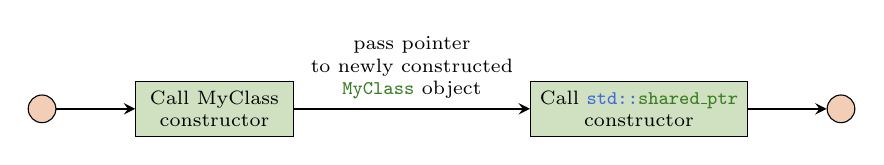
\begin{tikzpicture}
      \node[startnode] (start) {};
      \node[process] (p1) [right=1cm of start] {
          Call \lstinline!MyClass! \\ constructor
      };
      \node[process] (p2) [right=3cm of p1] {
        Call \sharedptr \\ constructor
      };
      \node[stopnode] (stop) [right=1cm of p2] {};

      \draw[flowarrow] (start.east) -- (p1.west);
      \draw[flowarrow] (p1.east) -- (p2.west) node [above,align=center,midway,font=\scriptsize]
      {
        pass pointer\\
        to newly constructed\\
        \object{MyClass} object
      };
      \draw[flowarrow] (p2.east) -- (stop.west);
    \end{tikzpicture}
  \end{center}

  \vspace{1ex}

  The constructors are called separately and the compiler cannot optimise memory location.

\end{frame}

\begin{frame}[fragile]
  \frametitle{Problems with explicit \object{new}'s: {\texttt\#2}}

  \begin{lstlisting}
void ProcessObject(std::shared_ptr<MyClass> obj, 
                   int process_id);

ProcessObject(std::shared_ptr<MyClass>(new MyClass()), 
              GetProcessID());
  \end{lstlisting}

  {\centering 
    \begin{tikzpicture}[tip/.style={->,shorten >=1pt, >=stealth},
                        every join/.style={rounded corners},
                        hv path/.style={to path={-| (\tikztotarget)}},
                        vh path/.style={to path={|- (\tikztotarget)}}]
                        %scale=.8, every node/.style={scale=.8}]
      \node[startnode] (start) {};
      \node[process] (p11) [below=10mm of start, xshift=-2.25cm,anchor=center] {\object{MyClass} \\ constructor};
      \node[process] (p12) [below=10mm of start, xshift=2.25cm, anchor=center] {\lstinline!GetProcessID()!};
      \node[process] (p21) [below=10mm of p11, xshift=-1.5cm, anchor=center] {\sharedptr \\ constructor};
      
      \only<1>{
        \node[process] (p22) [below=10mm of p11, xshift=1.5cm, anchor=center] {\lstinline!GetProcessID()!};
      }

      \only<2>{
        \node[dangerprocess] (p22) [below=10mm of p11, xshift=1.5cm, anchor=center] {\lstinline!GetProcessID()!};
      }
      \node[process] (p23) [below=10mm of p12, anchor=center] {\object{MyClass} \\ constructor};
      \node[process] (p31) [below=10mm of p21, anchor=center] {\lstinline!GetProcessID()!};
      \node[process] (p32) [below=10mm of p22, xshift=1.5cm, anchor=center] {\sharedptr \\ constructor};
      \node[stopnode] (stop) [below=10mm of p31, xshift=2.25cm, anchor=center] {};

      \coordinate[below=2mm of start] (startm) {};
      \coordinate[below=3mm of p11] (p1m) {};
      \coordinate[above=3mm of p32] (p32m) {};
      \coordinate[above=4mm of stop] (stopm) {};

      { [start chain]
        \chainin (start);
        \chainin (startm) [join];
        { [start branch=p12]
          \chainin (p12) [join=by {hv path, tip}];
          \chainin (p23) [join=by tip];
          \chainin (p32m) [join=by vh path];
        }
        \chainin (p11) [join=by {hv path, tip}];
        \chainin (p1m) [join];
        { [start branch=p22]
          \chainin(p22) [join=by {hv path, tip}];
          \chainin(p32m) [join=by vh path];
          \chainin (p32) [join=by tip];
          \chainin(stopm) [join=by vh path];
        }
        \chainin (p21) [join=by {hv path, tip}];
        \chainin (p31) [join=by tip];
        \chainin (stopm) [join=by vh path];
        \chainin (stop) [join=by tip];
      }

    \end{tikzpicture}
  \par}

  \note<2>
  {
    We have no control over the order in which the compiler carries out the three processes (other than that 
    calling \object{MyClass}'s creator has to happen before \sharedptr{}'s).
  }
\end{frame}

\begin{frame}[fragile]
  \frametitle{Create using \std{make\_unique} and \std{make\_shared}}

  Both these problems can be remedied by using \std{make\_shared} and \std{make\_unique} ({\footnotesize \emph{C++14}}).

  \vspace{1em}

  \begin{exampleblock}{Replacing the constructor call}
    \begin{lstlisting}
    void ProcessObject(std::shared_ptr<MyClass> obj, 
                       int process_id);

    ProcessObject(std::make_shared<MyClass>(), 
                  GetProcessID());
    \end{lstlisting}
  \end{exampleblock}

  \vspace{1em}

  Constructor calls cannot be intertwined with the \function{GetProcessID()} anymore.

  \note
  {
    On top of fixing these types of issues, using \function{make\_shared} and \function{make\_unique}
    doesn't reveal the underlying pointer, and therefore one cannot misuse the raw pointer without
    actively calling \function{.get()} or \function{.release()}, in which case it is easy to spot ones 
    mistakes.
  }

\end{frame}

\begin{frame}[fragile]
  \frametitle{Create using \std{make\_unique} and \std{make\_shared}}

  \begin{quoteblock}{Guideline}[Herb Sutter \cite{gotw89}]
    \begin{quote}
      Don't use explicit new, delete, and owning * pointers, except in rare cases 
      encapsulated inside the implementation of a low-level data structure.
    \end{quote}
  \end{quoteblock}

\end{frame}

\begin{frame}[fragile]
  \frametitle{Match constructors with destructors}

  Smart pointers have a control block which also keeps track of an allocator and a deleter

  \begin{exampleblock}{{\sharedptr{}} {\color{codeblockcolor}constructor}}
  \begin{lstlisting}
template <class Type, class Deleter, class Alloc>
std::shared_ptr(Type * p, Deleter d, Alloc a);
  \end{lstlisting}
  \end{exampleblock}

  \begin{exampleblock}{Custom deleter}
    \begin{lstlisting}[escapeinside={(*}{*)}]
std::shared_ptr<int> ap(new int[10]);(*\tikzmark{nodeleter}*)

std::shared_ptr<int> ap(new int[10], (*\tikzmark{withdeleter}*)
  std::default_delete<int[]>());

std::shared_ptr<int[]> ap(new int[10]);(*\tikzmark{specdeleter}*)
    \end{lstlisting}
  \end{exampleblock}

  \begin{tikzpicture}[overlay, remember picture]
    \draw[<-,>=stealth, font=\scriptsize] ($(nodeleter) + (.1em,.4ex)$) -- +(1,0) node[right] 
    {
      \begin{varwidth}{2cm}
        Destructs using \object{delete}
      \end{varwidth}
    };

    \draw[<-,>=stealth, font=\scriptsize] ($(withdeleter) + (.1em,-.4ex)$) -- +(1,0) node[right] 
    {
      \begin{varwidth}{2cm}
        Destructs using \lstinline!delete[]!
      \end{varwidth}
    };

    \draw[<-,>=stealth, font=\scriptsize] ($(specdeleter) + (.1em,.4ex)$) -- +(.65,0) node[right] 
    {
      \begin{varwidth}{2cm}
        Destructs using \lstinline!delete[]!
      \end{varwidth}
    };
  \end{tikzpicture}

  Very important that the deleter doesn't throw.

\end{frame}

\begin{frame}[fragile]
  \frametitle{Passing smart pointers}

  There are many options for passing smart pointers to functions (and classes).

  \vspace{1em}
  
  \begin{exampleblock}{Passing smart pointers}
    \begin{lstlisting}
void foo(MyClass *);
void foo(MyClass &);
void foo(std::unique_ptr<MyClass>);
void foo(std::unique_ptr<MyClass> &);
void foo(std::shared_ptr<MyClass>);
void foo(std::shared_ptr<MyClass> &);
    \end{lstlisting}
  \end{exampleblock}

  \vspace{1em}

  All of these has a distinct meaning, use them to express yourself.

  \note
  {
    Pointer vs reference boils down to the usual "Is no-value a valid option?", and in 
    classes pointers can be rebound, references not. Passing smart pointers by reference
    limits the function to only accept one type of smart pointers, while passing
    shared pointers by value has a cost (as the object needs to be constructed and 
    destructed).
  }

\end{frame}

\begin{frame}[fragile]
  \frametitle{Smart pointers and polymorphic classes}

  Using smart pointers and polymorphic classes as template arguments works as expected
  because one of the smart pointer constructors read:

  \vspace{1em}
  
  \begin{exampleblock}{The \sharedptr{} {\color{codeblockcolor}constructor}}
    \begin{lstlisting}
    template<class T, class U>
    std::shared_ptr<T>(const std::shared_ptr<U> &)
    \end{lstlisting}
  \end{exampleblock}

  \vspace{1em}

  This costructor can be used to convert between \sharedptr{}'s if \object{U*} is implicitly convertible to \object{T*}.

\end{frame}

\begin{frame}[fragile]
  \frametitle{Smart pointers and polymorphic classes}

  Assume we have a class hierarchy:

  \vspace{1em}

  \begin{center}
    \begin{tikzpicture}[scale=.6, every node/.style={scale=.6}]
      \umlclass[x=0,y=0]{Base}{}{void print();\\void print() const;}
      \umlclass[x=0,y=-4]{Derived}{}{void print();\\void sum();}
      \umlinherit{Base}{Derived}
    \end{tikzpicture}
  \end{center}

  \vspace{1em}

  Where \object{Derived} overloads the \function{print()} function but not the \object{const} variant.

\end{frame}

\begin{frame}[fragile]
  \frametitle{Smart pointers and polymorphic classes}

  \begin{lstlisting}[escapeinside={(*}{*)}]
std::shared_ptr<Derived> d_ptr = 
  std::make_shared<Derived>();

std::shared_ptr<Base> b_ptr = d_ptr;
std::shared_ptr<const Base> b_const_ptr = d_ptr;

std::shared_ptr<Derived> d_err_ptr = b_ptr;(*\tikzmark{dfromb}*)
std::shared_ptr<Base> b_err_ptr = b_const_ptr;(*\tikzmark{bfrombc}*)

b_ptr->print();(*\tikzmark{bdprint}*)
b_const_ptr->print();(*\tikzmark{bdcprint}*)

//use_count: 3
  \end{lstlisting}

  \begin{tikzpicture}[overlay, remember picture]
    \draw[<-,>=stealth, font=\scriptsize] ($(dfromb) + (.1em,.4ex)$) -- +(1,0) node[right,red!50!black] {Compilation error};
    \draw[<-,>=stealth, font=\scriptsize] ($(bfrombc) + (.1em,.4ex)$) -- +(.48,0) node[right,red!50!black] {Compilation error};
    \draw[<-,>=stealth, font=\scriptsize] ($(bdprint) + (.1em,.4ex)$) -- +(2,0) node[right] (end)
    {
      Calls \lstinline!Derived::print()!
    };
    \coordinate (begin) at ($(bdcprint) + (.1em,.4ex)$);
    \draw[<-,>=stealth, font=\scriptsize] (begin) -- (begin -| end.west) node[right]
    {
      Calls \lstinline!Base::print() const!
    };
  \end{tikzpicture}

\end{frame}

\begin{frame}[fragile]
  \frametitle{Smart pointers and polymorphic classes}

  \begin{lstlisting}[escapeinside={(*}{*)}]
std::shared_ptr<Derived> d_ptr = 
  std::make_shared<Derived>();

std::shared_ptr<Base> b_ptr = d_ptr;
std::shared_ptr<const Base> b_const_ptr = d_ptr;

std::shared_ptr<Derived> d_new_ptr = 
  std::dynamic_pointer_cast<Derived>(b_ptr);(*\tikzmark{dfrombN}*)

std::shared_ptr<Base> b_new_ptr = 
  std::const_pointer_cast<Base>(b_const_ptr);(*\tikzmark{bfrombcN}*)

d_new_ptr->sum();(*\tikzmark{dsum}*)
b_new_ptr->print();(*\tikzmark{bnewprint}*)

//use_count: 5
  \end{lstlisting}

  \begin{tikzpicture}[overlay, remember picture]
    \draw[<-,>=stealth, font=\scriptsize] ($(dfrombN) + (.1em,.4ex)$) -- +(1,0) node[right] (ok1) {OK!};
    \coordinate (bfstart) at ($(bfrombcN) + (.1em,.4ex)$);
    \draw[<-,>=stealth, font=\scriptsize] (bfstart) -- (bfstart -| ok1.west) node[right] {OK!};
    
    \draw[<-,>=stealth, font=\scriptsize] ($(dsum) + (.1em,.4ex)$) -- +(1,0) node[right] (dsum)
    {
      Calls \lstinline!Derived::sum()!
    };

    \coordinate (bnewbegin) at ($(bnewprint) + (.1em,.4ex)$);
    \draw[<-,>=stealth, font=\scriptsize] (bnewbegin) -- (bnewbegin -| dsum.west) node[right]
    {
      Calls \lstinline!Derived::print()!
    };
  \end{tikzpicture}

  \note
  {
    This is a more error safe way of working with pointer casts as one never has to access
    the underlying raw pointer and explicitly own raw pointers as one would have to do
    with \lstinline!.get()! together with standard C++ casts. It would also not be possible to
    re-own the result of the standard cast as one has extraced it out of the reference counting
    object. This is inteded to use with \sharedptr{}'s, and doesn't work with \uniqueptr{}.
  }

\end{frame}

\begin{frame}
  \frametitle{Smart pointers and the STL}

  \begin{itemize}
    \item Smart pointers can be stored in the STL containers.
    \item However, not all algorithms work with the resulting containers.
    \begin{itemize}
      \item E.g. \uniqueptr{} is MoveConstructible and MoveAssignable
      \item But not CopyConstructable or CopyAssignable
    \end{itemize}
  \end{itemize}

  \vspace{1em}

  Thus if an algorithm requires CopyConstructability and a \uniqueptr{} is given, 
  it should fail to compile.

  \vspace{1em}

  \autoptr{} on the other hand is a bit more unreliable.

  \note
  {
    \autoptr{} is technically not CopyConstructable and CopyAssignable as the copied
    object is changed, but this won't always result in a compilation error (or even
    a compilation warning) as it should. It depends on your compiler, but is not a 
    risk one should take regardless. Before the introduction of move semantics 
    for example, an iterator needed to be CopyConstructable and assignable for
    it to be used with the sort-algorithm. auto\_ptr's would therefore
    not be usable in this case, but not all compilers would warn you of that.
  }

\end{frame}

\begin{frame}
  \frametitle{The boost pointer container library}

  Library inteded to provide a STL-like library for single ownership pointers.

  \begin{block}{Advantages}
    \begin{itemize}
      \item Simplifies the container-of-pointer syntax.
      \item Notational convenience
        \begin{itemize}
          \item Dereferencing an iterator returns a dereferenced pointer
        \end{itemize}
      \item Introduces ``Clonability'' to do deep copies.
      \item Faster and has a small memory overhead.
    \end{itemize}
  \end{block}

  \begin{alertblock}{Disadvantages}
    \begin{itemize}
      \item Not very compatible with the algorithm library
      \item Not as flexible as a container of smart pointers
    \end{itemize}
  \end{alertblock}

\end{frame}

\begin{frame}
  \frametitle{Summary}

  \begin{itemize} \setlength\itemsep{2em}
    \item Use smart pointers to manage dynamic resources so that they are freed when they aren't used anymore.
      \begin{itemize} \setlength\itemsep{1em}
        \item Use \uniqueptr{} to signal singular ownership
        \item Use \sharedptr{} to signal shared ownership
        \item Use \weakptr{} to signal uncommitted shared ownership
      \end{itemize}
    \item Avoid using explicit \object{new} and \object{delete} statements, and explicit ownership of raw pointers.
  \end{itemize}

\end{frame}

\end{document}
